\documentclass[11pt]{article}
\usepackage[top=1cm, bottom=2cm]{geometry}                % See geometry.pdf to learn the layout options. There are lots.
\geometry{a4paper}                   % ... or a4paper or a5paper or ... 
%\geometry{landscape}                % Activate for for rotated page geometry
%\usepackage[parfill]{parskip}    % Activate to begin paragraphs with an empty line rather than an indent
\usepackage{graphicx}
\usepackage{amsmath, amsthm, amssymb}
\usepackage{epstopdf}
\DeclareGraphicsRule{.tif}{png}{.png}{`convert #1 `dirname #1`/`basename #1 .tif`.png}

\title{Chapter 13   Independence}
%\author{Doug Stirling}
\date{}                                           % Activate to display a given date or no date


\usepackage{titlesec}
\titlespacing*{\subsubsection}{0pt}{20pt}{7pt}
\titlespacing*{\subsection}{0pt}{30pt}{7pt}

\begin{document}
\maketitle

\section{Probability and applications}
\subsection{Joint probabilities}

\subsubsection*{Data sets with two categorical variables}

Bivariate categorical data sets are usually summarised with a contingency table.

For example, a study examined 686 tourists and classified each by educational level and by whether they were `information seekers' (who requested destination-specific literature from travel agents) or `non-seekers':

\begin{center}
\begin{tabular}{lrrr}
&\multicolumn{2}{c} {\textbf{Information seeker?}} \\
\textbf{Education}	    &\multicolumn{1}{c}{\textbf{Yes} }   	    &\multicolumn{1}{c}{\textbf{No} }   	   &\textbf{Total}   \\  \cline{2-3}
\quad Some high school	&\multicolumn{1}{|r}{13}	&\multicolumn{1}{r|}{27}	&40 \\
\quad High school degree   	&\multicolumn{1}{|r}{64}	&\multicolumn{1}{r|}{118}	&182 \\
\quad Some college   	&\multicolumn{1}{|r}{100}	&\multicolumn{1}{r|}{123}	&223 \\
\quad College degree   	&\multicolumn{1}{|r}{59}	&\multicolumn{1}{r|}{69}	&128 \\
\quad Graduate degree   	&\multicolumn{1}{|r}{67}	&\multicolumn{1}{r|}{46}	&113 \\ \cline{2-3}
\textbf{Total} &303	&383	&686
\end{tabular}
\end{center}

\subsubsection*{Joint probabilities}

Bivariate categorical data can be modelled as a random sample from an underlying population of pairs of categorical values. The population proportion for each pair (x, y) is denoted by pxy and is called the joint probability for (x, y).

In games of chance, we can often work out the joint probabilities. For example, if a gambler draws a card from a shuffled deck and also tosses a coin, there are eight possible combinations,

\begin{center}
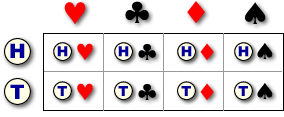
\includegraphics[scale=0.75]{images/prob/cardAndCoin}
\end{center}

Since these are equally likely,

\[p_{head, heart}  =  p_{head, club}  =  ...  =  p_{tail, spade}  =  \frac 18  =  0.125 \]

\subsubsection*{Interest in the model}

In practice, we usually only have a random sample (summarised by a contingency table) and do not know the underlying joint probabilities. The sample proportions however provide \textbf{estimates}.

\begin{center}
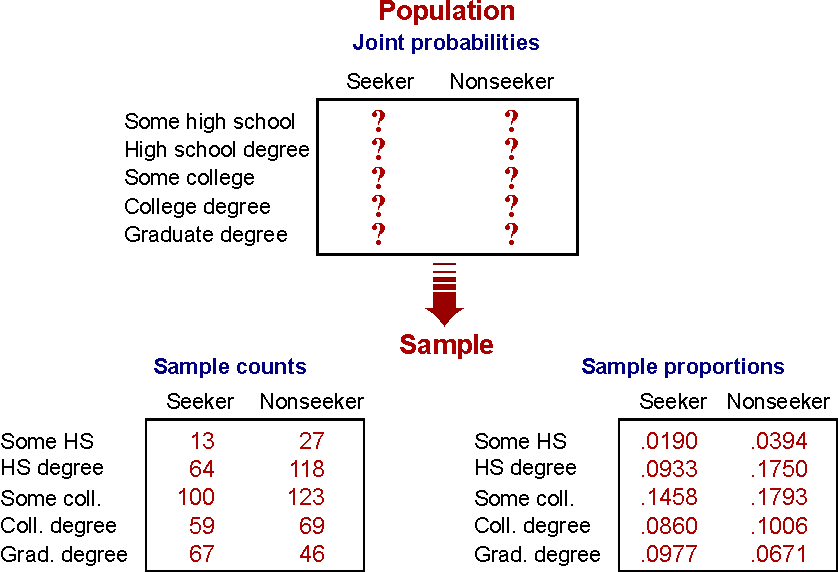
\includegraphics[scale=0.75]{images/prob/seekers}
\end{center}


\subsection{Marginal probabilities}

\subsubsection*{Probabilities for a single variable}

A model for two categorical variables is characterised by the joint probabilities $p_{xy}$.

The \textbf{marginal probability}, $p_x$, for a variable X is the proportion of $(x, y)$ pairs in the population with $X  = x$ . This can be found by adding all joint probabilities for pairs with this x-value.




\end{document}  